\documentclass[11pt]{article}
\usepackage[margin=1in]{geometry}
\usepackage{graphicx}
\usepackage{booktabs}
\usepackage{hyperref}
\usepackage{float}
\usepackage[T1]{fontenc}

\title{GEPA Prompt Evolution Analysis\\\large Run: \texttt{claude\_sonnet46}}
\author{Auto-generated from \texttt{reports/generate\_report.py}}
\date{2026-04-24}

\begin{document}
\maketitle

\section{Overview}
This report inspects a single GEPA run that optimized the system prompt for a
Bitcoin forward-looking sentiment scoring task (1--15 scale). GEPA
(reflective prompt optimization) iteratively proposes a new prompt by having a
reflection LM read trajectories and evaluator feedback on a minibatch of
training examples, then accepts the proposal if it improves on the parent
candidate on the minibatch~\cite{gepa}. Related prompt-optimization
approaches include APE~\cite{ape}, PromptBreeder~\cite{promptbreeder}, and
DSPy/COPRO~\cite{dspy}.

\section{Run summary}
\begin{center}
\begin{tabular}{lr}
\toprule
Metric & Value \\
\midrule
Candidates (final pool size) & 11 \\
Iterations logged            & 15 \\
Reflection LM calls          & 14 \\
Seed prompt words            & 92 \\
Best candidate words         & 1669 \\
Word-count growth factor     & 18.14x \\
Jaccard(best, seed)          & 0.33 \\
\bottomrule
\end{tabular}
\end{center}

\section{Prompt length evolution}
GEPA reflective mutation typically \emph{grows} prompts by appending
structured guidance (headers, rules, worked examples). Figure~\ref{fig:len}
shows the word and character count per candidate.
\begin{figure}[H]\centering
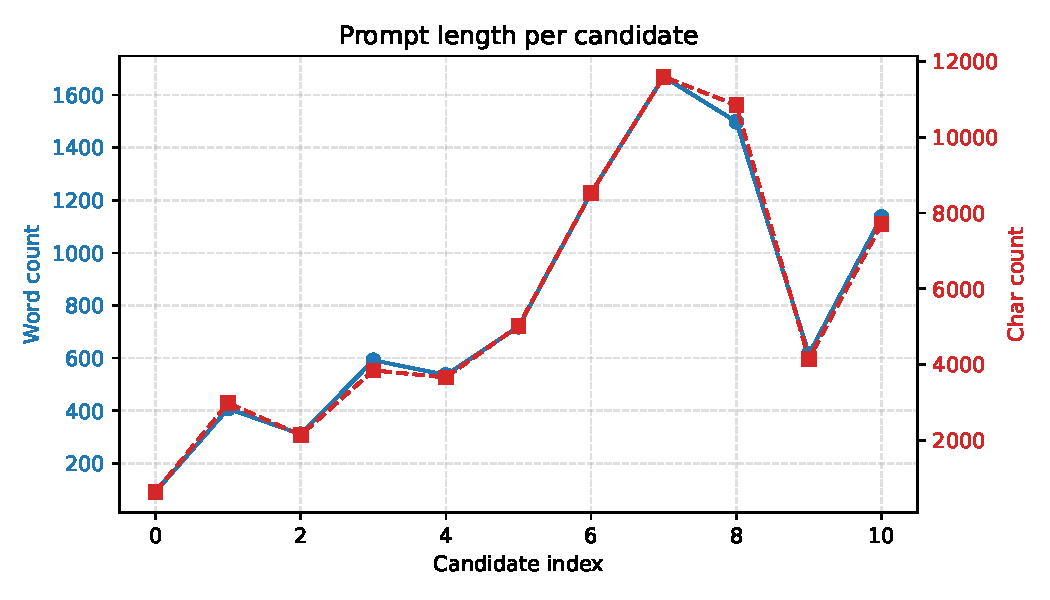
\includegraphics[width=\linewidth]{figures/prompt_length.pdf}
\caption{Prompt length per candidate (words, chars).}
\label{fig:len}
\end{figure}

\section{Lexical drift from seed}
Jaccard token overlap measures how much each candidate departs from the seed's
vocabulary. Low values indicate the reflection LM has introduced a substantial
new vocabulary, consistent with instruction-densification.
\begin{figure}[H]\centering
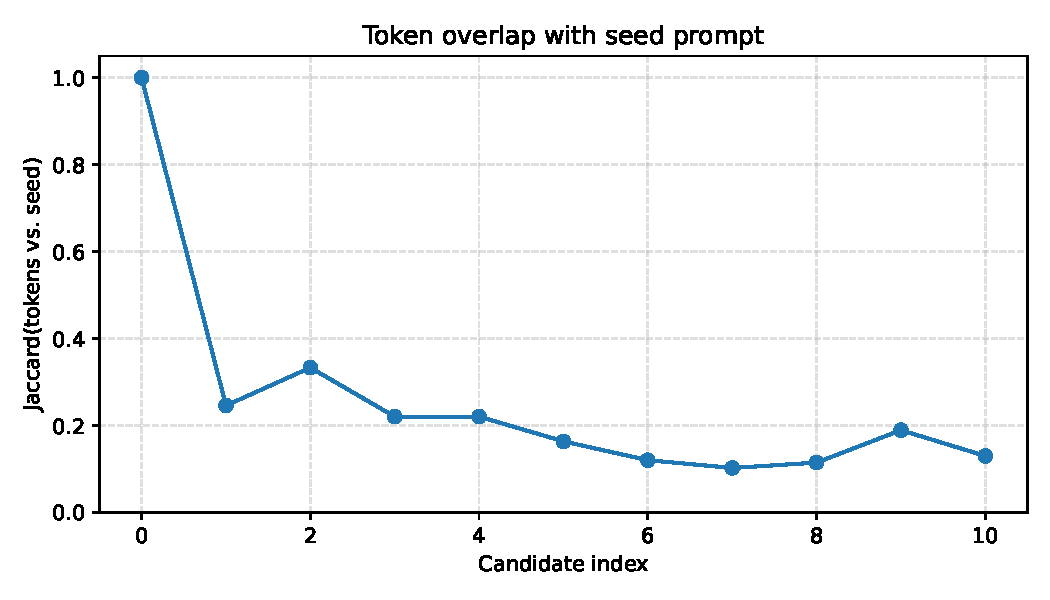
\includegraphics[width=0.85\linewidth]{figures/jaccard_vs_seed.pdf}
\caption{Jaccard(candidate tokens, seed tokens).}
\end{figure}

\section{Structural features over time}
Prompt optimization often converges on a \emph{format}: headers, bullet
lists, numbered steps, tables, and fenced code blocks for output
specification. Figure~\ref{fig:struct} tracks these structural features per
candidate.
\begin{figure}[H]\centering
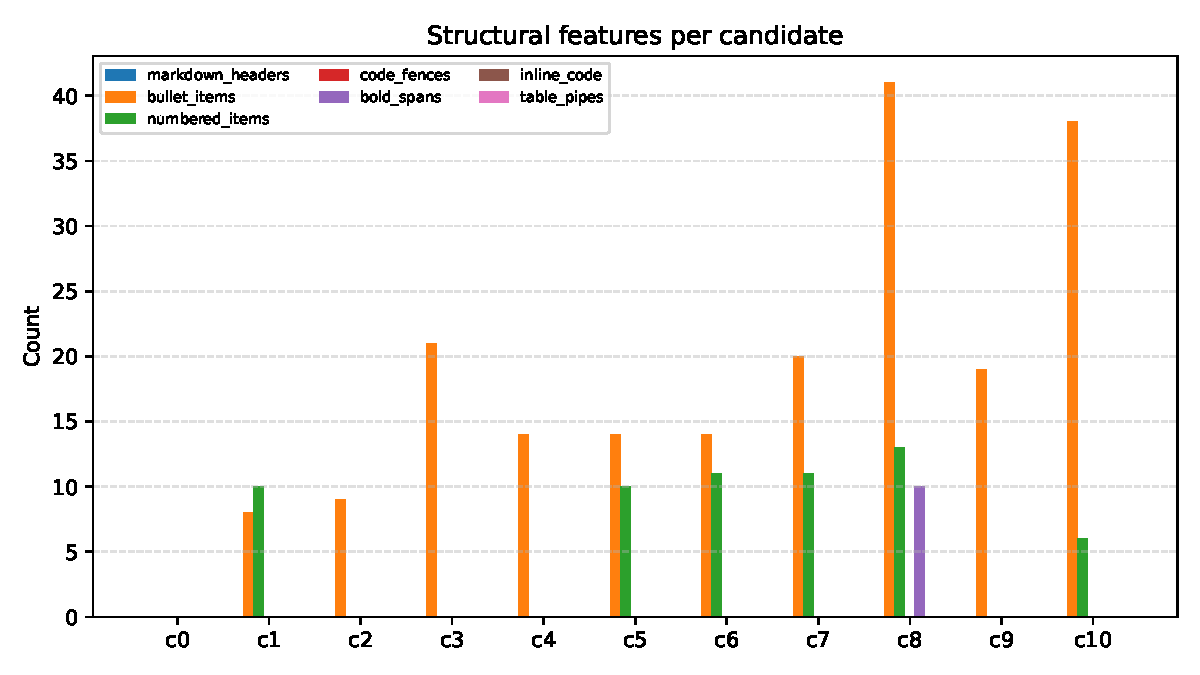
\includegraphics[width=\linewidth]{figures/structural_features.pdf}
\caption{Structural feature counts per candidate.}
\label{fig:struct}
\end{figure}

\section{Domain-keyword heatmap}
A fixed lexicon of Bitcoin-sentiment domain terms, tracked per candidate,
exposes which semantic axes GEPA emphasizes over iterations.
\begin{figure}[H]\centering
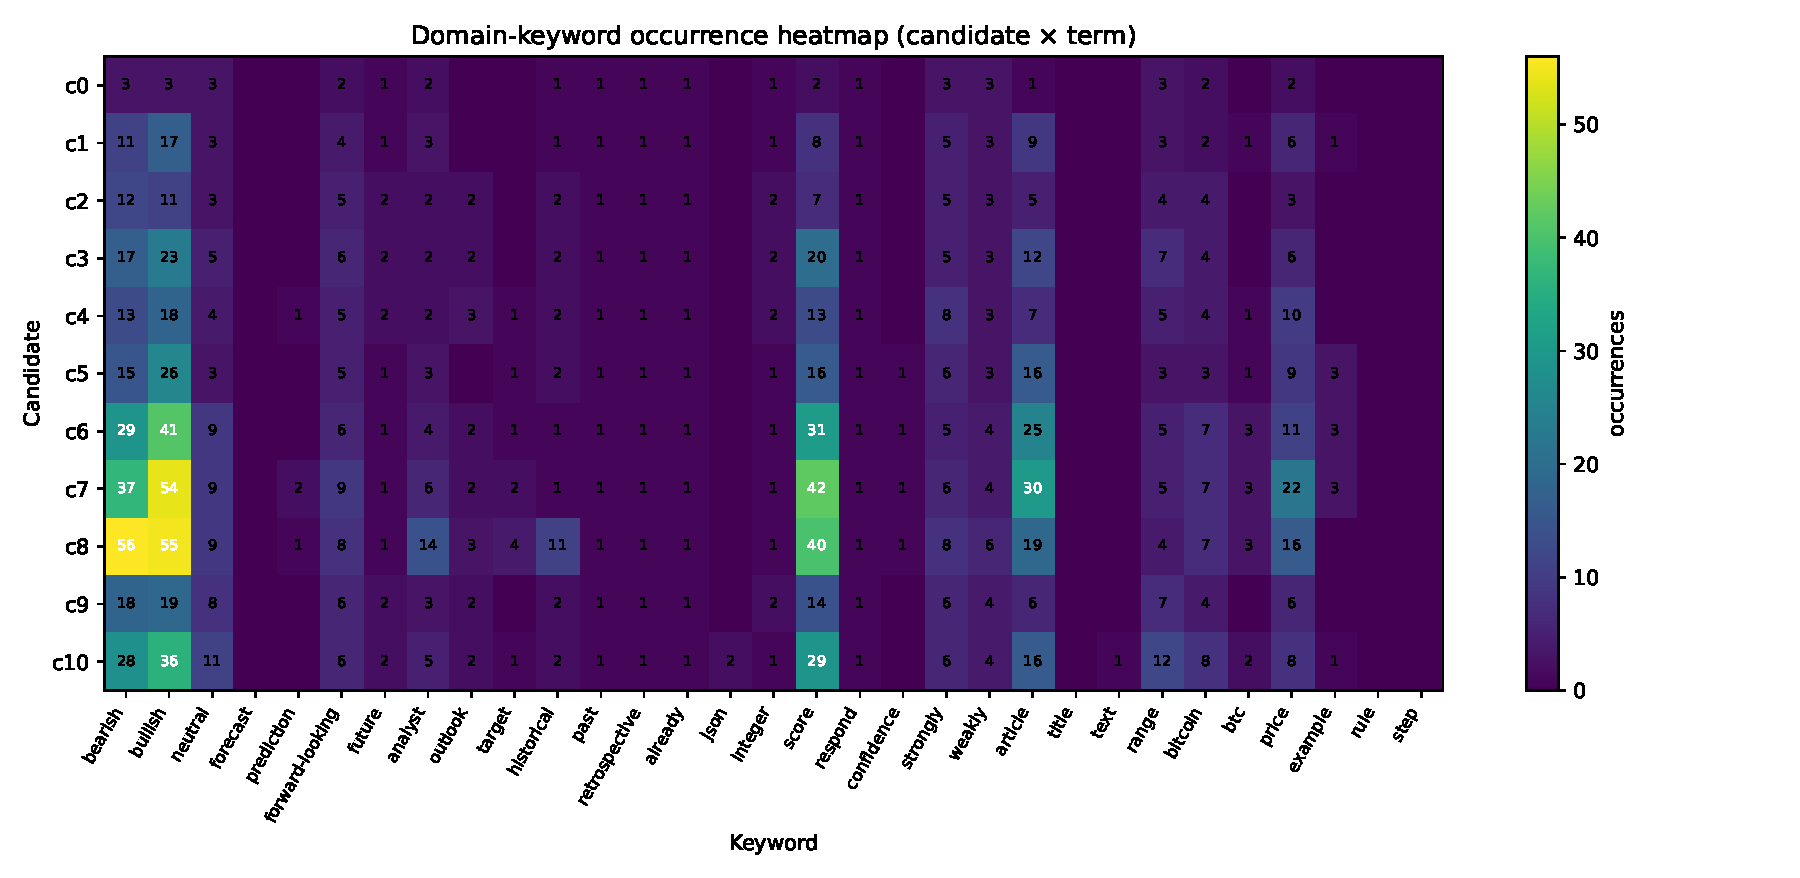
\includegraphics[width=\linewidth]{figures/keyword_heatmap.pdf}
\caption{Domain-keyword occurrence heatmap (candidate $\times$ term).}
\end{figure}

\section{New tokens introduced by GEPA}
Tokens present in at least one mutated candidate but absent from the seed.
This is a first-order readout of what the reflection LM is \emph{adding}.
\begin{figure}[H]\centering
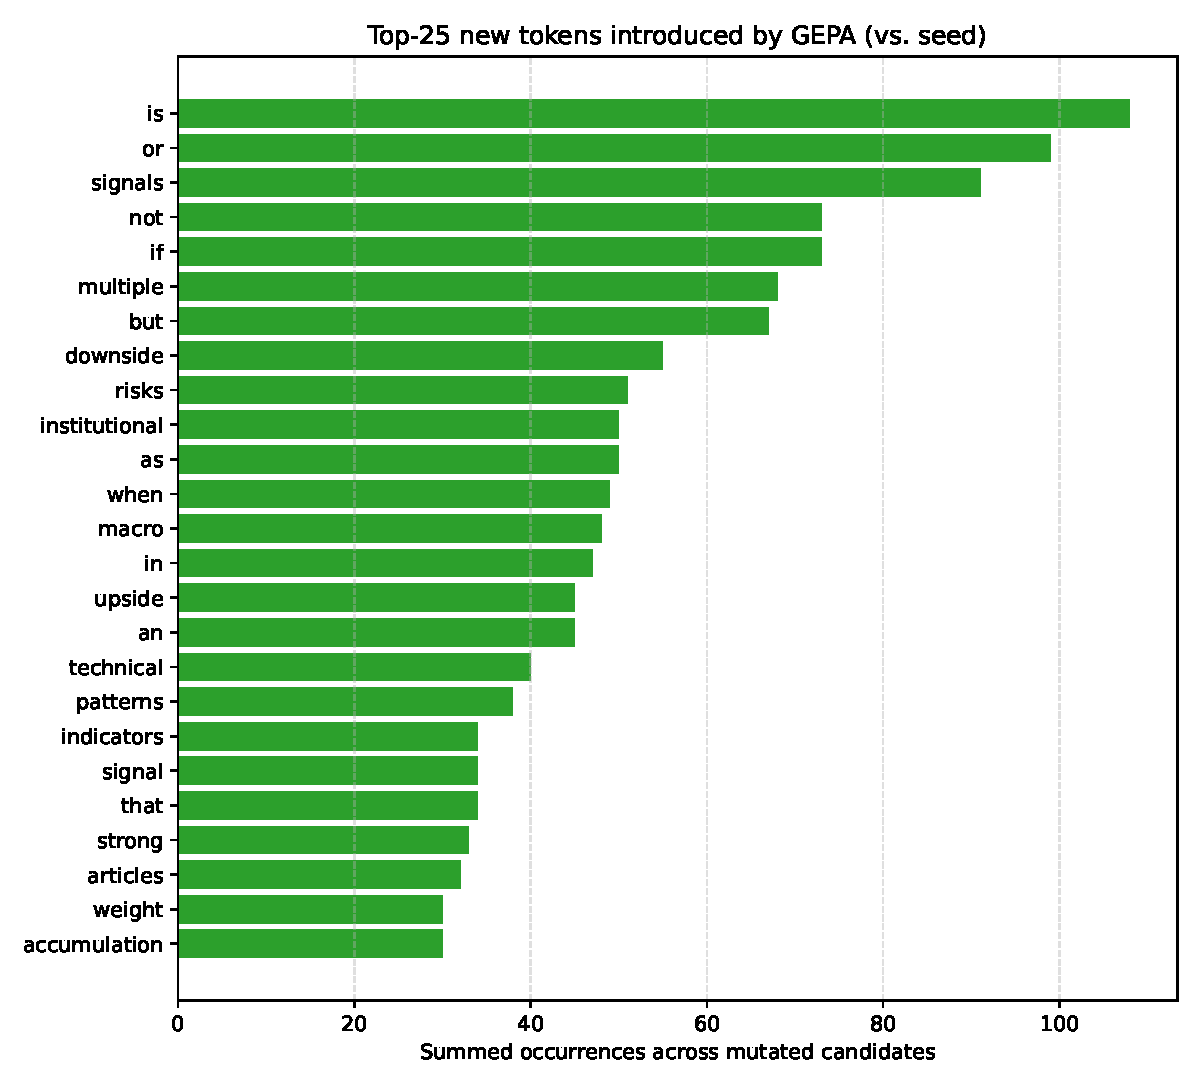
\includegraphics[width=0.9\linewidth]{figures/new_tokens.pdf}
\caption{Top new tokens introduced vs.\ seed.}
\end{figure}

\section{Iteration dynamics}
GEPA's acceptance criterion compares the proposed candidate's mean score on
the sampled minibatch against the parent's mean score. Vertical bars mark
accepted proposals.
\begin{figure}[H]\centering
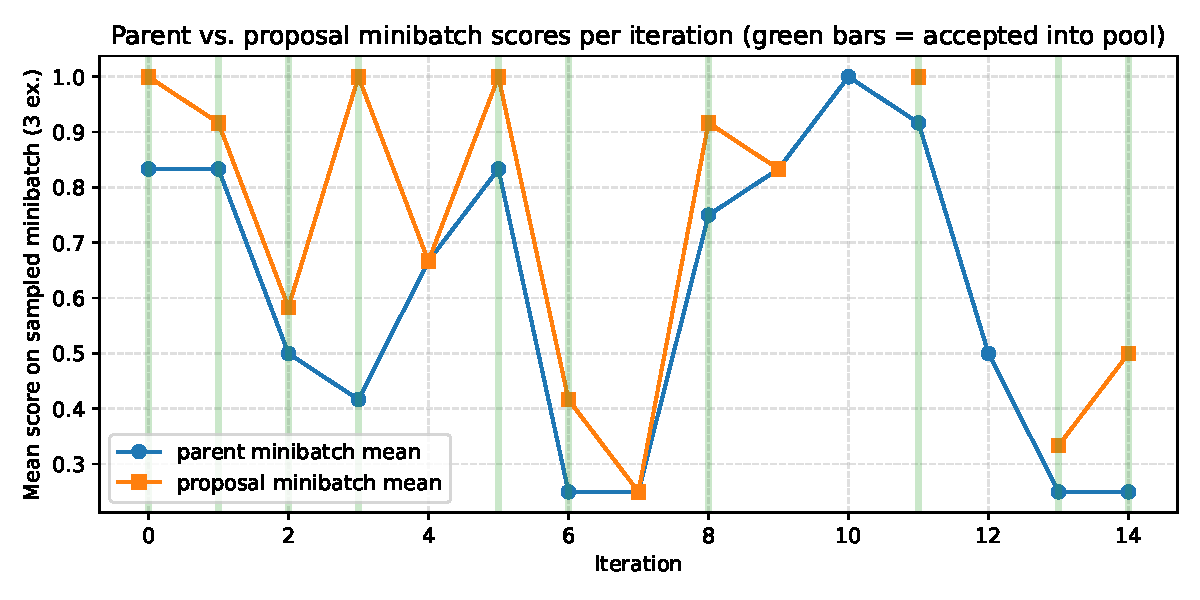
\includegraphics[width=\linewidth]{figures/iteration_scores.pdf}
\caption{Parent vs.\ proposal minibatch scores.}
\end{figure}

\begin{figure}[H]\centering
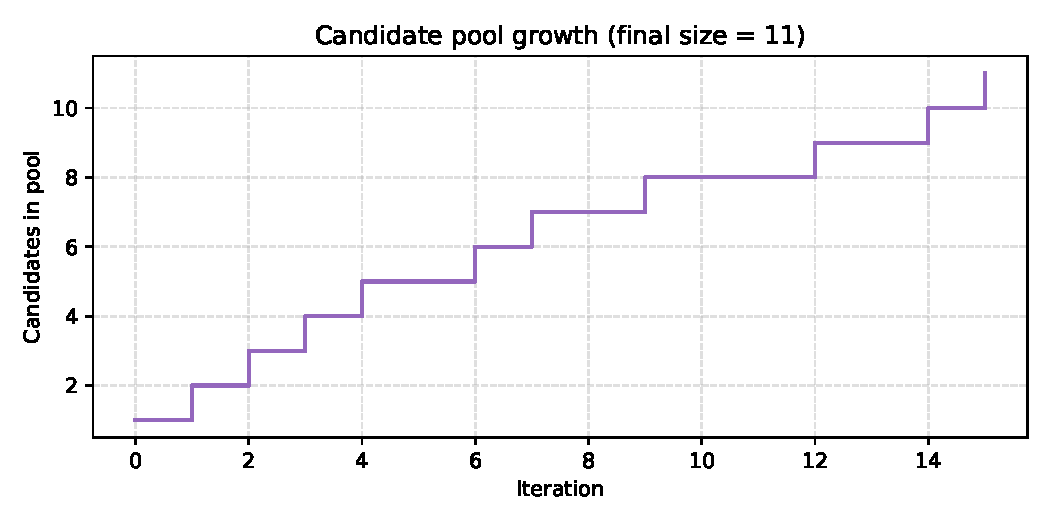
\includegraphics[width=0.85\linewidth]{figures/pool_growth.pdf}
\caption{Candidate pool growth (Pareto-admissible set size).}
\end{figure}

\section{Per-task score heatmap}
For every accepted candidate, GEPA stores the best model output per valset
task. Re-scoring these outputs against the gold labels exposes which examples
a new prompt fixed or broke, which is more informative than the aggregate
valset score alone.
\begin{figure}[H]\centering
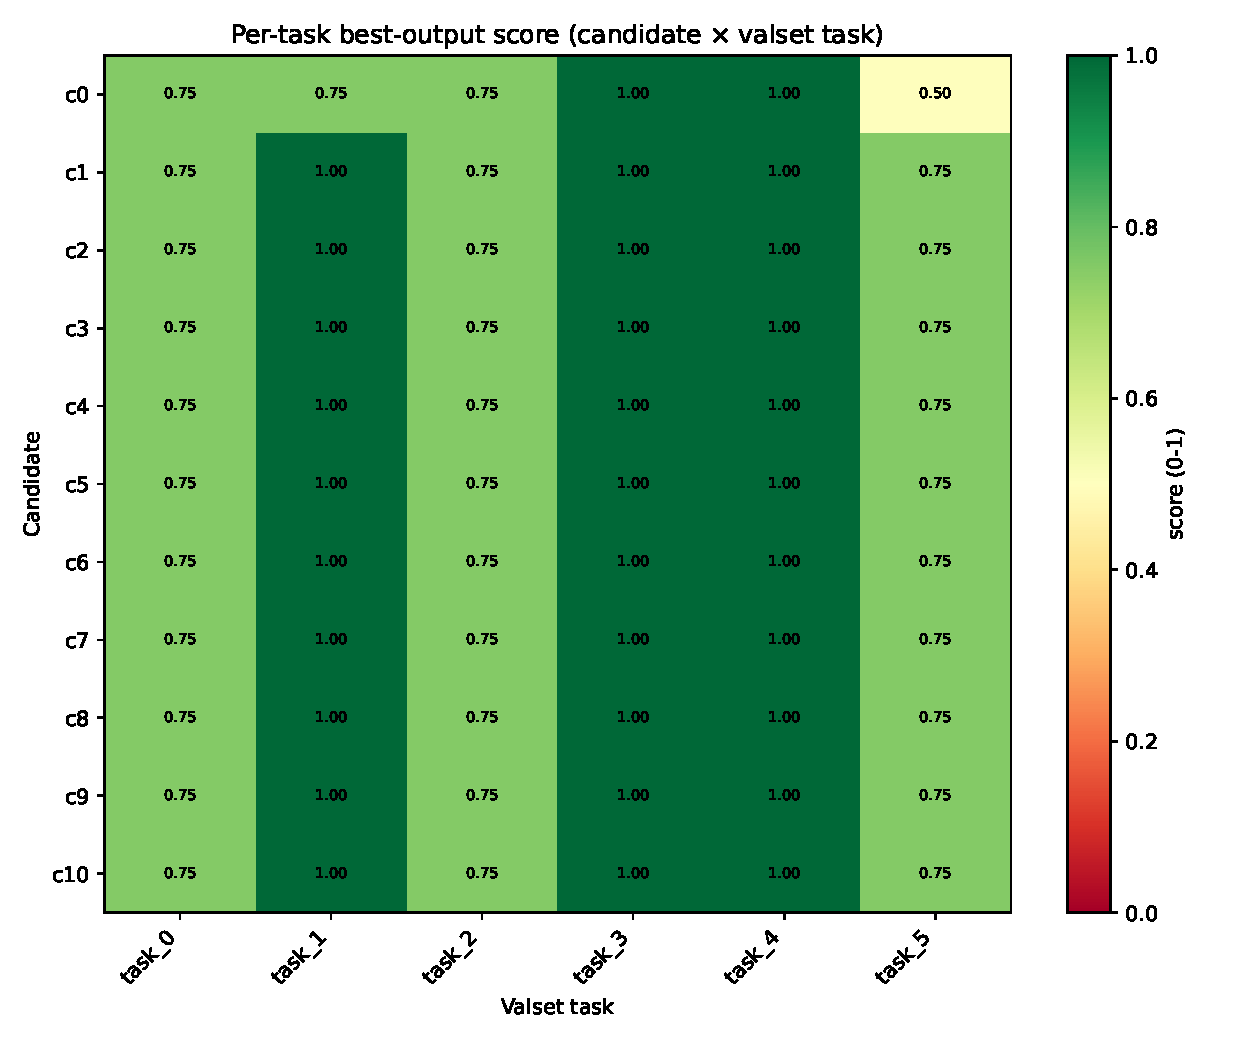
\includegraphics[width=\linewidth]{figures/per_task_heatmap.pdf}
\caption{Per-task best-output score per candidate.}
\end{figure}

\section{Reflection LM cost}
The reflection LM consumes a large prompt (full trajectory + evaluator
feedback) and returns a new candidate plus rationale. These plots expose how
context size grows across calls.
\begin{figure}[H]\centering
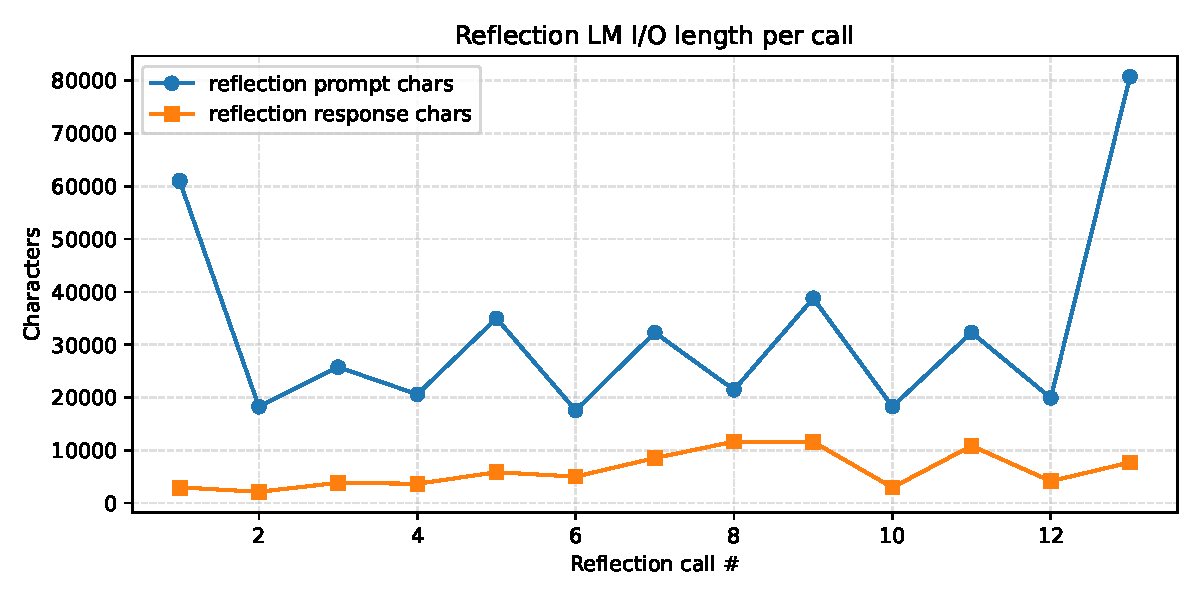
\includegraphics[width=\linewidth]{figures/reflection_length.pdf}
\caption{Reflection LM prompt and response lengths.}
\end{figure}
\begin{figure}[H]\centering
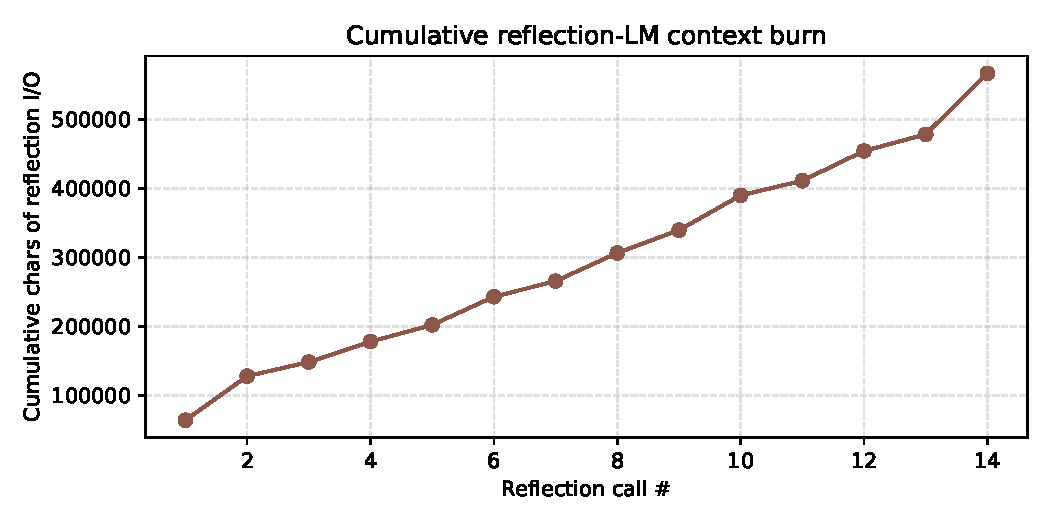
\includegraphics[width=0.85\linewidth]{figures/reflection_cumulative.pdf}
\caption{Cumulative reflection-LM context burn.}
\end{figure}

\begin{thebibliography}{9}
\bibitem{gepa} GEPA: Reflective Prompt Optimization (Python package,
  \url{https://github.com/gepa-ai/gepa}).
\bibitem{ape} Zhou et al., Large Language Models Are Human-Level Prompt
  Engineers (APE), 2022.
\bibitem{promptbreeder} Fernando et al., PromptBreeder: Self-Referential
  Self-Improvement via Prompt Evolution, 2023.
\bibitem{dspy} Khattab et al., DSPy: Compiling Declarative Language Model
  Calls into Self-Improving Pipelines, 2024.
\end{thebibliography}

\end{document}
